%%%%%%%%%%%%%%%%%%%%%%%%%%%%%%%%%%%%%%%%%%%%%%%%%%%%%%%%%%%%%%%%%%%%%%%%%%%

\documentclass[a4paper,oneside,12pt]{article}
\usepackage{mystyle}

\begin{document}

\title{\Large\bf Cartesian coordinate system}
\author{%%
  Minh Van Nguyen \\
  \url{mvngu@gmx.com}
}
\date{\today}
\maketitle


%%%%%%%%%%%%%%%%%%%%%%%%%%%%%%%%%%%%%%%%%%%%%%%%%%%%%%%%%%%%%%%%%%%%%%%%%%%

\section{Coordinates}

Let's start by discussing how a pair of numbers can be represented as
a picture.  You know that any real number can be represented as a
point on the number line.  \Figure{fig:real_number_line} shows the
irrational numbers $\sqrt{2}$, $e$, and $\pi$ as points on the number
line.  What if you have a pair $\tuple{a}{b}$ of real numbers?  How
would $\tuple{a}{b}$ be represented as a point on the number line?

\begin{figure}[!htbp]
\centering
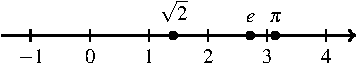
\includegraphics[scale=1.1]{image/03/number-line.pdf}
\caption{%%
  Elements from the set $\RR$ of real numbers can be represented as
  points on the number line.
}
\label{fig:real_number_line}
\end{figure}

The answer is that a pair $\tuple{a}{b}$ of real numbers cannot be
represented as a point on the number line.  You must somehow extend
the number line.  One way to extend the number line is to draw a
vertical line through the point $0$ such that the vertical line is
perpendicular to the number line.  What you then obtain is the
\emph{Cartesian coordinate system} as shown in
\Figure{fig:Cartesian_coordinate_system}.  In the Cartesian coordinate
system, a pair $\tuple{a}{b}$ of real numbers can be represented as a
point with the pair $\tuple{a}{b}$ being now called a pair of
\emph{coordinates}.  The number $a$ in the coordinates $\tuple{a}{b}$
is called the $x$-coordinate because starting from $0$ on the
$x$-axis you must move a horizontal distance of $a$ units to get to
the coordinates $\tuple{a}{0}$.  The number $b$ in the coordinates
$\tuple{a}{b}$ is called the $y$-coordinate because starting from $0$
on the $y$-axis you must move a vertical distance of $b$ units to get
to the coordinates $\tuple{0}{b}$.  Add the coordinates $\tuple{a}{0}$
and $\tuple{0}{b}$ together and you get the coordinates
$\tuple{a}{b}$, which can be drawn as a point in the Cartesian
coordinate system.

\begin{figure}[!htbp]
\centering
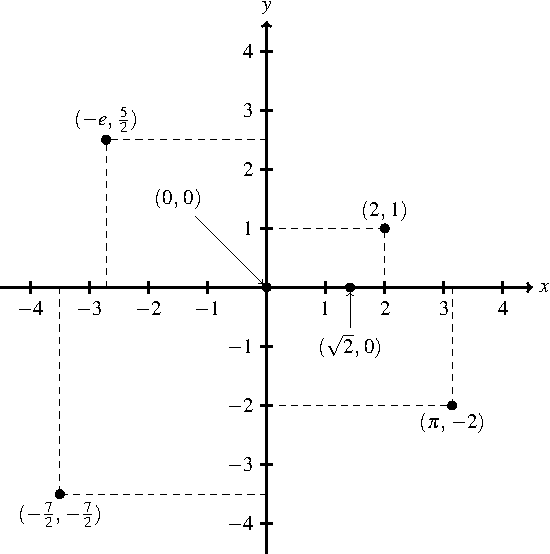
\includegraphics[scale=1.1]{image/03/cartesian-coordinate.pdf}
\caption{%%
  The Cartesian coordinate system consists of two perpendicular axes
  called the $x$-axis and the $y$-axis.  A pair $\tuple{a}{b}$ of real
  numbers can be represented as a point.  Starting from the origin
  $\tuple{0}{0}$, you move a distance of $a$ units along the
  horizontal axis and then move $b$ units along the vertical axis.
  Where you end up is the point $\tuple{a}{b}$.
}
\label{fig:Cartesian_coordinate_system}
\end{figure}

\begin{exercise}
Represent the pairs $\tuple{2}{4}$, $\tuple{0}{-3}$, and
$\tuple{-4}{0}$ as points in the Cartesian coordinate system.
\end{exercise}

\ifbool{showSolution}{
\begin{solution}
See \Figure{fig:some_points_in_Cartesian_coordinate_system}.
%%
\begin{figure}[!htbp]
\centering
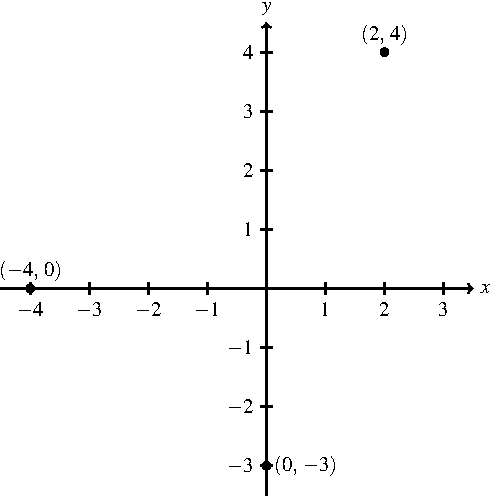
\includegraphics[scale=1.1]{image/03/cartesian-coordinate_2-5_0-3_4-0.pdf}
\caption{%%
  The pairs $\tuple{2}{4}$, $\tuple{0}{-3}$, and $\tuple{-4}{0}$ as
  points in the Cartesian coordinate system.
}
\label{fig:some_points_in_Cartesian_coordinate_system}
\end{figure}
\end{solution}
}{}


%%%%%%%%%%%%%%%%%%%%%%%%%%%%%%%%%%%%%%%%%%%%%%%%%%%%%%%%%%%%%%%%%%%%%%%%%%%

\section{Distance}

The distance between two points $A$ and $B$ is the length of the
straight line from $A$ to $B$.  In the Cartesian coordinate system,
you use the same technique to measure the distance between two
points.  Suppose the points $A$ and $B$ have coordinates
$A = \tuple{x_1}{y_1}$ and $B = \tuple{x_2}{y_2}$; see
\Figure{fig:distance_between_two_points}.  If $A \neq B$, then there
is a third point $C$ with coordinates $C = \tuple{x_1}{y_2}$.  The
line segments $AC$, $BC$, and $AB$ are the three sides of a
right-angled triangle.  The segment $AC$ has length
\[
a
=
\absoluteValue{y_1 - y_2}
=
\absoluteValue{y_2 - y_1}
\]
and the segment $BC$ has length
\[
b
=
\absoluteValue{x_2 - x_1}
=
\absoluteValue{x_1 - x_2}
\]
but you do not yet know the length of the segment $AB$.  However,
since the points $\triple{A}{B}{C}$ are the three corners of a
right-angled triangle, you can use Pythagoras' theorem to determine
the length of the segment $AB$.

\begin{theorem}
\textbf{Pythagoras' theorem.}
Let $\triple{a}{b}{c}$ be the lengths of the three sides of a
right-angled triangle, where $c$ is the length of the hypotenuse.
Then $c$ can be written as $a^2 + b^2 = c^2$.
\end{theorem}

\begin{figure}[!htbp]
\centering
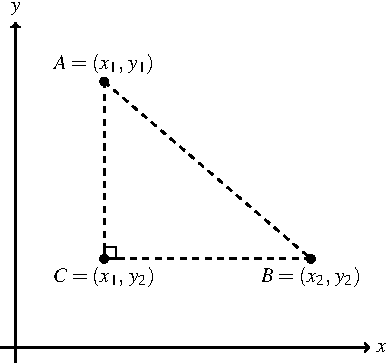
\includegraphics[scale=1.1]{image/03/distance-two-points.pdf}
\caption{%%
  Any two distinct points $A$ and $B$ are two corners of a
  right-angled triangle.  The line segment $AB$ is the hypotenuse,
  whose length can be measured by Pythagoras' theorem.
}
\label{fig:distance_between_two_points}
\end{figure}

Let $c$ be the length of the segment $AB$.  Use Pythagoras' theorem to
write
%%
\begin{align*}
c^2
&=
a^2 + b^2 \\[4pt]
&=
\absoluteValue{y_2 - y_1}^2 + \absoluteValue{x_2 - x_1}^2 \\[4pt]
&=
(y_2 - y_1)^2 + (x_2 - x_1)^2.
\end{align*}
%%
Solve the last expression for $c$ and you obtain
\[
c
=
\sqrt{
  (y_2 - y_1)^2
  +
  (x_2 - x_1)^2
}
\]
which proves the following theorem.

\begin{theorem}
\label{thm:distance_between_two_points}
Let $A = \tuple{x_1}{y_1}$ and $B = \tuple{x_2}{y_2}$ be two points in
the Cartesian coordinate system.  If $A \neq B$, then the distance
between $A$ and $B$ can be written as
\[
\sqrt{
  (y_2 - y_1)^2
  +
  (x_2 - x_1)^2
}.
\]
\end{theorem}

\begin{exercise}
Consider the points $(\sqrt{2}\comma 0)$ and $\tuple{2}{1}$ from
\Figure{fig:Cartesian_coordinate_system}.  Determine the distance
between those two points.
\end{exercise}

\ifbool{showSolution}{
\begin{solution}
Use \Theorem{thm:distance_between_two_points} to write
%%
\begin{align*}
\sqrt{
  (1 - 0)^2
  +
  (2 - \sqrt{2})^2
}
&=
\sqrt{
  1^2 + (2 - \sqrt{2})^2
} \\[4pt]
&\approx
1.3431
\end{align*}
%%
correct to four decimal places.  The symbol ``$\approx$'' means
``approximately''.  In other words, the distance between the points
$(\sqrt{2}\comma 0)$ and $\tuple{2}{1}$ is approximately $1.3431$.
\end{solution}
}{}

\end{document}
